\documentclass[border=10pt]{standalone}
\usepackage{pgfplots}
\pgfplotsset{compat=1.18}
\begin{document}
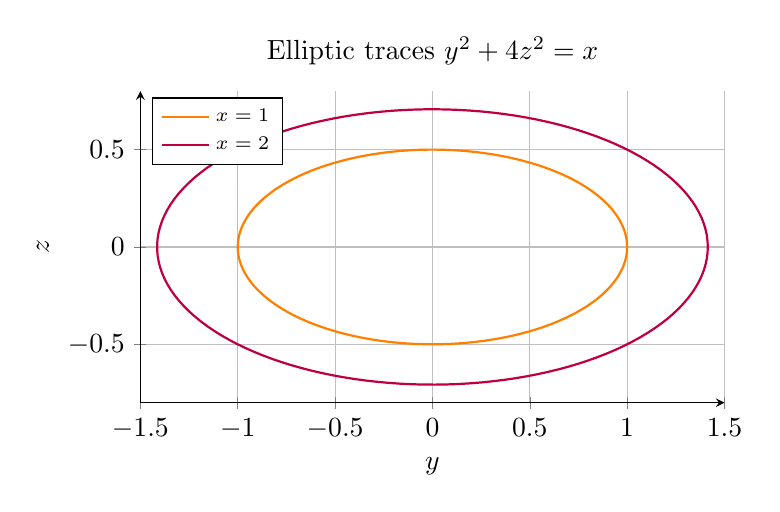
\begin{tikzpicture}
\begin{axis}[
  width=9cm, height=8cm,
  xlabel={$y$}, ylabel={$z$},
  xmin=-1.5, xmax=1.5, ymin=-0.8, ymax=0.8,
  grid=major,
  axis lines=left,
  axis equal image,
  legend style={at={(0.02,0.98)}, anchor=north west, font=\scriptsize},
  title={Elliptic traces $y^2+4z^2=x$},
]
\addplot[orange, thick, domain=0:360, samples=150] ({sqrt(1)*cos(x)},{0.5*sqrt(1)*sin(x)});
\addlegendentry{$x=1$}
\addplot[purple, thick, domain=0:360, samples=150] ({sqrt(2)*cos(x)},{0.5*sqrt(2)*sin(x)});
\addlegendentry{$x=2$}
\end{axis}
\end{tikzpicture}
\end{document}